\documentclass[12pt]{article}

\usepackage[utf8]{inputenc}
\usepackage{geometry}
\geometry{
    a4paper,
    total={170mm,257mm},
    left=25mm,
    right=25mm,
    top=25mm,
    bottom=25mm,
}
\usepackage{multicol}
\usepackage[font=small,labelfont=bf]{caption}
\setlength{\columnsep}{0.25cm}
\usepackage[inline]{enumitem}
\usepackage{amssymb}
\usepackage{xcolor}
\usepackage{mathtools} 
\setlength{\parindent}{0em}
\setlength{\parsep}{0em}
\usepackage{tikz}
\setlength{\parskip}{0em}
\usetikzlibrary{decorations.pathmorphing,patterns}
\usepackage[american,cuteinductors]{circuitikz}
\usetikzlibrary{shapes,arrows,circuits,calc,babel}
% Definition of blocks:
\tikzset{%
  block/.style    = {draw, thick, rectangle, minimum height = 3em,
    minimum width = 3em},
  sum/.style      = {draw, circle, node distance = 2cm}, % Adder
  input/.style    = {coordinate}, % Input
  output/.style   = {coordinate} % Output
}
% Defining string as labels of certain blocks.
\newcommand{\suma}{\Large$+$}
\newcommand{\inte}{$\displaystyle \int$}
\newcommand{\derv}{\huge$\frac{d}{dt}$}

\def\mf{\ensuremath\mathbf}
\def\mb{\ensuremath\mathbb}
\def\mc{\ensuremath\mathcal}
\def\lp{\ensuremath\left(}
\def\rp{\ensuremath\right)}
\def\lv{\ensuremath\left\lvert}
\def\rv{\ensuremath\right\rvert}
\def\lV{\ensuremath\left\lVert}
\def\rV{\ensuremath\right\rVert}
\def\lc{\ensuremath\left\{}
\def\rc{\ensuremath\right\}}
\def\ls{\ensuremath\left[}
\def\rs{\ensuremath\right]}
\def\bmx{\ensuremath\begin{bmatrix*}[r]}
\def\emx{\ensuremath\end{bmatrix*}}
\def\bmxc{\ensuremath\begin{bmatrix*}[c]}
\def\emxc{\ensuremath\end{bmatrix*}}
% \def\t{\lp t\rp}
% \def\k{\ls k\rs}

\newcommand{\demoex}[2]{\onslide<#1->\begin{color}{black!60} #2 \end{color}}
\newcommand{\demoexc}[3]{\onslide<#1->\begin{color}{#2} #3 \end{color}}
\newcommand{\anim}[3]{\onslide<#1->{\begin{color}{#2!60} #3 \end{color}}}
\newcommand{\ct}[1]{\lp #1\rp}
\newcommand{\dt}[1]{\ls #1\rs}

% \renewcommand{\familydefault}{\sfdefault}

\begin{document}
\begin{center}
\begin{large}
\textbf{Applied Linear Algebra in Data Analaysis}\\
\vspace{0.1cm}
\end{large}
\textbf{Solutions to Linear Equations Assignment}
\end{center}
\hrule
\vspace{1em}

\begin{large}
    \textbf{Marks: 31}
\end{large}
\vspace{0.2cm}

\textbf{Note}: The questions you need to answer are written down in red for clarity for some of the problems.

\begin{enumerate}
\item Derive force and displacement relationship for a series of $n+1$ springs (with spring constants $k_i$) connected in a line. There are $n$ nodes, with $f_i$ and $x_i$ representing the force applied and resulting displacement at the $i^{th}$ node. 
\begin{center}
    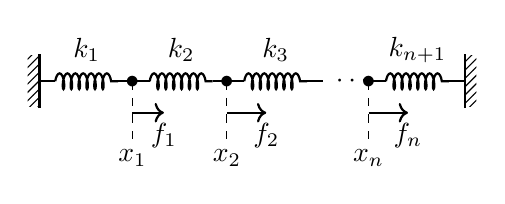
\begin{tikzpicture}
        \fill [pattern = north east lines] (-0.15,-0.325) rectangle (0,0.325);
        \draw[thick] (0,-0.34) -- (0,0.34);

        \draw[thick] (0,0) -- (0.2,0);
        \draw[decoration={aspect=0.3, segment length=1mm, amplitude=1mm, coil,},decorate, thick] (0.2,0) -- (1.0,0);
        \draw[thick] (1.0,0) -- (1.2,0);
        \node[black] at (1.18,-0.02) {$\bullet$};
        \node[black] at (0.6,0.4) {$k_1$};
        \draw[dashed, thin] (1.18,0) -- (1.18,-0.75) node[below]{$x_1$};
        \draw[->,thick] (1.18,-0.4) -- (1.58,-0.4) node[below]{$f_1$};

        
        \draw[thick] (1.2,0) -- (1.4,0);
        \draw[decoration={aspect=0.3, segment length=1mm, amplitude=1mm, coil,},decorate, thick] (1.4,0) -- (2.2,0);
        \draw[thick] (2.2,0) -- (2.4,0);
        \node[black] at (2.38,-0.02) {$\bullet$};
        \node[black] at (1.8,0.4) {$k_2$};
        \draw[dashed, thin] (2.38,0) -- (2.38,-0.75) node[below]{$x_2$};
        \draw[->,thick] (2.38,-0.4) -- (2.88,-0.4) node[below]{$f_2$};
        
        \draw[thick] (2.4,0) -- (2.6,0);
        \draw[decoration={aspect=0.3, segment length=1mm, amplitude=1mm, coil,},decorate, thick] (2.6,0) -- (3.4,0);
        \draw[thick] (3.4,0) -- (3.6,0);
        \node[black] at (3.0,0.4) {$k_3$};

        \node[black] at (4.0, 0) {$\cdots$};

        \draw[thick] (4.2,0) -- (4.4,0);
        \draw[decoration={aspect=0.3, segment length=1mm, amplitude=1mm, coil,},decorate, thick] (4.4,0) -- (5.2,0);
        \draw[thick] (5.2,0) -- (5.4,0);
        \node[black] at (4.18,-0.02) {$\bullet$};
        \node[black] at (4.8,0.4) {$k_{n+1}$};
        \draw[dashed, thin] (4.18,0) -- (4.18,-0.75) node[below]{$x_n$};
        \draw[->,thick] (4.18,-0.4) -- (4.68,-0.4) node[below]{$f_n$};

        \fill [pattern = north east lines] (5.4,-0.325) rectangle (5.55,0.325);
        \draw[thick] (5.4,-0.34) -- (5.4,0.34);
    \end{tikzpicture}
\end{center}
\textcolor{red}{
\begin{enumerate}
    \item Represent the relationship in the following form, \textbf{[Marks: 2]}
    \[ \mf{f} = \mf{Kx}; \,\,\, \mf{f} = \begin{bmatrix}f_1\\ f_2\\ \vdots\\ f_n\end{bmatrix}; \,\,\, \mf{x} = \begin{bmatrix}x_1 \\ x_2 \\ \vdots \\ x_n\end{bmatrix}\]
    \item What kind of a pattern does $\mf{K}$ have? \textbf{[Marks: 1]}
    \item \textcolor{blue}{\textbf{[Programming]}} Consider a specific case where $n = 4$ and $k = 1.5 N.m^{-1}$. What should be forces applied at the four nodes in order to displace the spring $\mf{x} = \begin{bmatrix*} 0.5 \\ -0.5 \\ 0 \\ 0 \end{bmatrix*}m$. \textbf{[Marks: 4]} 
\end{enumerate}
}

\item Consider the following electrical circuit with rectangular grid of resistors $R$. The input to this grid is a set of current injected at the top node as shown in the figure, such that $\sum_{k=1}^5i_k = 0$.
\vspace{-0.25cm}
\begin{center}
\begin{circuitikz}[scale=0.9]
    \draw (2,0) to[R,*-*] (0,0)
    to[R,*-*] (0,2) to[R,*-*] (0,4) to[R,*-*] (2,4)
    to[R,*-*] (2,2) to[R,*-*] (2,0) to[R,*-*] (4,0)
    to[R,*-*] (4,2) to[R,*-*] (4,4) to[R,*-*] (6,4)
    to[R,*-*] (6,2) to[R,*-*] (6,0) to[R,*-*] (8,0)
    to[R,*-*] (8,2) to[R,*-*] (8,4) to[R,*-*] (6,4);

    \draw (0,2) to[R,*-*] (2,2);
    \draw (2,4) to[R,*-*] (4,4);
    \draw (2,2) to[R,*-*] (4,2);
    \draw (4,2) to[R,*-*] (6,2);
    \draw (4,0) to[R,*-*] (6,0);
    \draw (6,2) to[R,*-*] (8,2);

    \draw (0,5) node[above]{$i_1$} to[short, o-] (0,4);
    \draw (2,5) node[above]{$i_2$} to[short, o-] (2,4);
    \draw (4,5) node[above]{$i_3$} to[short, o-] (4,4);
    \draw (6,5) node[above]{$i_4$} to[short, o-] (6,4);
    \draw (8,5) node[above]{$i_5$} to[short, o-] (8,4);
\end{circuitikz}
\end{center}

\textcolor{red}{Express the relationship between the voltages at the different nodes (represented by $\bullet$ in the figure) and the net current flowing in/out of the node in the following form, $\mf{G}\mf{v} = \mf{i}$. Where, $\mf{G}$ is the conductance matrix, $\mf{v}$ is the vector of node voltages, and $\mf{i}$ is the vector representing the net current flow in/out of the different node. \textbf{[Marks: 3]}}

\item \textbf{Two point boundary problem.} $\mf{A}\mf{x} = \mf{b}$ is often encountered in many practical applications. One such application is the numerical solution of differential equations of the following form,
\[ \sum_{i=0}^M a_{i}\ct{x}y^{\ct{i}}\ct{x} = f\ct{x} \]
where, $x \in \dt{a, b}$ and $y\ct{a} = \alpha, y\ct{b} = \beta$. 

Numerical methods are often employed for obtaining an approximate estimate of $y\ct{x}$ at discrete points in the interval $\dt{a,b}$. The interval is divided into subintervals of width $\Delta x$. The derivate of $y\ct{x}$ at the different nodes (points between two subintervals) can be approximated as the following,
\begin{align}
y'\ct{x_i} &= \frac{y\ct{x_i + \Delta x} - y\ct{x_i - \Delta x}}{\Delta x}\nonumber\\
y''\ct{x_i} &= \frac{y\ct{x_i + \Delta x} + 2y\ct{x_i} - y\ct{x_i - \Delta x}}{\Delta x^2} \nonumber
\end{align}
where, $x_i = a + i\Delta x, \,\, 0 \leq i \leq N+1$, and $b - a = \ct{N+1} \Delta x$. Addition and subtracting the above two equations and neglecting terms involving higher orders of $\Delta x$, we get the following approximations for the derivatives of $y\ct{x}$ at $x_i$.

Replacing the derivatives of $y\ct{x}$ by the above approximations and evaluating the equation at the different nodes $x_i$s, we arrive a set of $N$ linear equations with $N$ unknowns $y\ct{x_1}, y\ct{x_2}, \ldots y\ct{x_N}$. 

\textcolor{red}{Using this approach, compute an approximate solution for $y\ct{x}$ for the following differential equations over the interval $x \in \dt{0, 1}$.
\begin{enumerate}
        \item $y''\ct{x} = -x$
        \item $y''\ct{x} + y'\ct{x} = x$
\end{enumerate}
\textcolor{blue}{\textbf{[Programming]}} Solve these equations for different values of $\Delta x$, and compare the resulting approximate solution for $y\ct{x}$ with the exact solution.   Present your results as a plot the solution $y\ct{x_i}$ versus $x_i$. \textbf{[Marks: 4]}}

\textcolor{red}{Comment on the dependence of the solution $\ct{x}$ on $\Delta x$. What is the best value for $\Delta x$ to use in solving these equations? \textbf{[Marks: 2]}}

\item \textbf{Ill-conditioned systems.} A system $\mf{A}\mf{x} = \mf{b}$ is said to be ill-conditioned when small changes in the components of $\mf{A}$ or $\mf{b}$ can produce large changes in the solution $\mf{x}$. Consider the following system,
\begin{align}
x - y &= 100 \nonumber \\
10 + \ct{9 + \Delta}y &= 0 \nonumber
\end{align}
\textcolor{red}{\textcolor{blue}{\textbf{[Programming]}} Find the solutions of the system for different values of $\Delta = -2, -1, 0, 1, 2$. How do the solutions change with $\Delta$. \textbf{[Marks: 2]}} 

Now consider the following system,
\begin{align}
x - y &= 100 \nonumber \\
10 - \ct{9 + \Delta}y &= 0 \nonumber
\end{align}
\textcolor{red}{\textcolor{blue}{\textbf{[Programming]}} Find the solutions of the system for different values of $\Delta = -2, -1, 0, 1, 2$. How do the solutions change with $\Delta$. \textbf{[Marks: 2]}} 

The second system is an example of an ill-conditioned system. What can you say about the geometries of these two systems? \textbf{[Marks: 2]}

% \item \textbf{Connectivity matrices.} Another common application of matrices is in graph theory. A graph is a set of vertices or nodes connected by edges, as show in the following figure. $A$-$F$ are the nodes of the graph, and the lines with the arrows are the edges that convey information about the connections or relationships between the nodes.
% \begin{center}
%     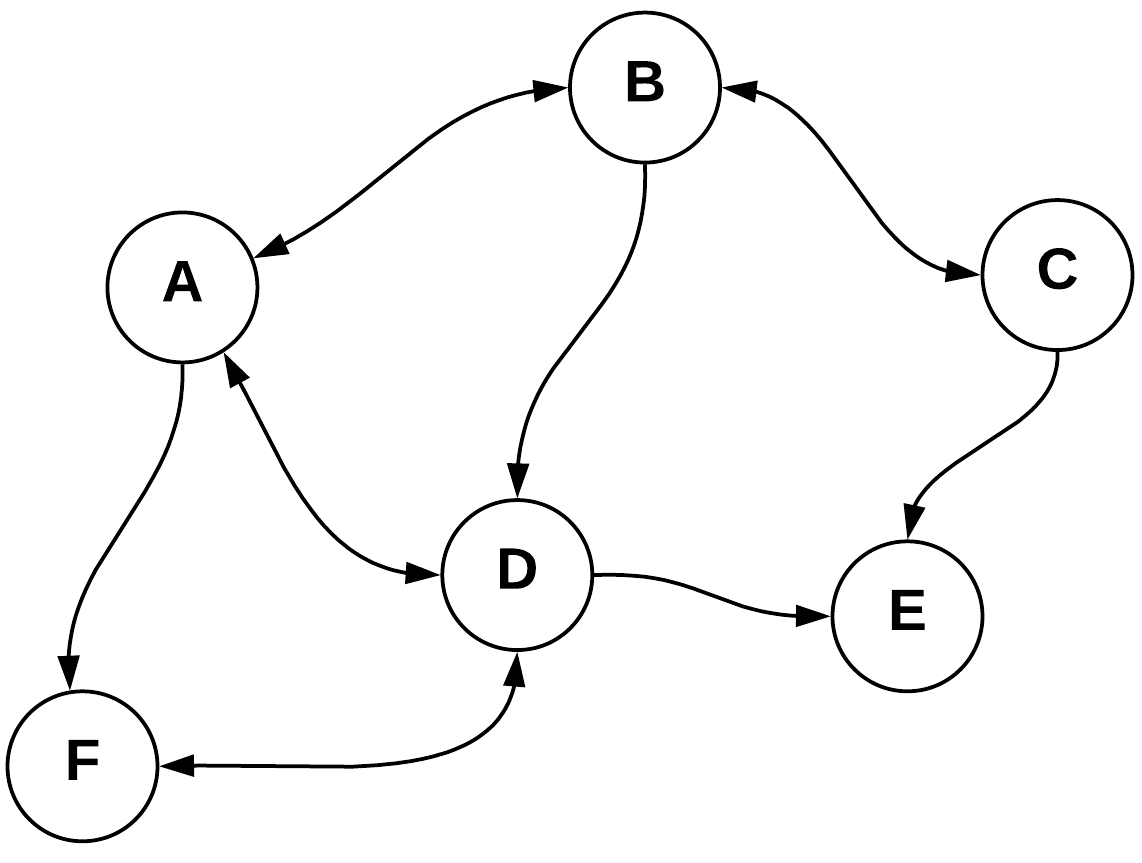
\includegraphics[width=0.5\columnwidth]{../figs/graph.png}
% \end{center}
% The above graph can be thought as a representation of different places in a city (represented by the nodes), and the lines with the arrows represent the roads connecting these different places. A line with two arrows allow two-way traffic, while line with single arrow only allow one way traffic. The connectivity between the different places can be summarized though the connectivity matrix $\mf{C} \in \mb{R}^{n \times n}$, where $n$ is the number of nodes in the graph. The elements of this connectivity matrix  represents whether or not there is a direct path between two places.
% \[ 
% c_{ij} = \begin{cases}
%     1 & \text{there is a direct road between places } i \, \& \,j. \\
%     0 & \text{otherwise.}
% \end{cases}
% \]
% The diagonal element of $\mf{C}$ are zero, $c_{ii} = 0$.

% Write down the connectivity matrix $\mf{C}$ for the graph shown above. How can we use the matrix $\mf{C}$ to answer the following questions? Explain exact matrix operation you would perform to answer these questions (Hint: Consider higher power of $\mf{C}$).
% \begin{enumerate}
%     \item Is there a path between two places $i$ and $j$ that goes via one other place? For example, we can go from $A$ to $D$ via $B$.
%     \item How many paths are there between places $i$ and $j$ that goes via three other places?
% \end{enumerate}

\item \textbf{Computed Tomography} (CT) is a medical imaging technique that is used to reconstruct the internal structure of an object from a set of X-ray measurements. The object is placed between an X-ray source and a detector. The X-ray source and the detector are rotated around the object, and the X-ray measurements are recorded at different angles. The X-ray measurements are then used to reconstruct the internal structure of the object.
\begin{figure}[h]
    \centering
    \includegraphics[width = 0.6\textwidth]{../../analysis/imaging/output/ct_setup_full.pdf}
    \caption{A simplified CT set-up with a single X-ray source and a single detector, that are located diametrically opposite to each other and can rotate to any scan angle $\phi$. The object is placed between the X-ray source and the detector, which is depicted by the gray square of side $l$. The x-ray originates from the green triangle (x-ray source), passes through the object, and is detected by the red triangle (detector). The x-ray undergoes attenuation as it passes through the object. Different points in the objects are most likely to have different attentuation coefficients, and the goal of CT is toe reconstruct of spatial map of the attentuation within the object, which provides a measure of the internal structure of the object.}
    \label{fig:ct}
\end{figure}

The x-ray attentuation equation is given by,
\[ I_o = I_i \exp\lp -\mu l \rp \]
where, $I_i$ is the intensity of the x-ray entering an object with fixed attentuation coefficient $\mu$, $I_o$ is the intensity of the x-ray existing the object, and $l$ is the path length of the x-ray in the object. 

In general, the attenuation coefficient is a function of the position within the object, $\mu = \mu\ct{x,y}$. The goal of CT is to reconstruct the spatial map of the attenuation coefficient $\mu\ct{x,y}$.

Let $L$ represent the line segment of the x-ray within the object as shown in Figure~\ref{fig:ct}, and the attentuation outside the object is assumed to be zero. If $I_s$ is the intensity of the x-ray leaving the source, the intensity of the x-ray reaching the detector $I_d$ is given by,
\[ I_d = I_s \exp\lp - \int_L \mu \ct{x, y} dl \rp \]
where, $dl$ is the differential length along the line segment $L$, which is a function of $x, y$. The integral in the above equation is the line integral of the attenuation coefficient $\mu\ct{x,y}$ along the line segment $L$.

We wish to solve this problem using a computer by posing it as a set of linear equations relating the attenuation coefficient $\mu\ct{x,y}$ to the x-ray intensity measurements $I_d$. For simplicity, we will assume $I_s = 1$. First, we simplify the above integration equation by taking the log on both sides, which results in,
\[ \ln I_d = - \int_L \mu \ct{x, y} dl \]
\textcolor{red}{Explain the why above step is valid. Do we need to worry about the case where $I_d = 0$? \textbf{[Marks: 2]}}

Discretize the object into $n \times n$ grid of pixels, and assume that attentuation coefficient within each pixel to be constant. For any given scan angle $\phi$ you need to find out the pixels the line segment $L$ passes through, along with the path length of the x-ray line segment within each pixel. \textcolor{red}{Derive the discrete expression relating the x-ray intensity measurements $I_d$ to the attenuation coefficient $\mu\ct{x,y}$ for a given scan angle $\phi$, assuming a discretized object $n \times n$. Write down the above expression in the following form \textbf{[Marks: 3]},
\[ \tilde{\mf{a}}\ct{\phi}^\top \mf{x} = y\ct{\phi} \]}
where, $\mf{x} \in \mb{R}^{n^2}$ is the vector of unknown attenuation coefficients of the pixels in the image, $\tilde{\mf{a}}\ct{\phi} \in \mb{R}^{n^2}$ is the vector relating the attentuation coefficients to the detector measurement for the given source-detector angle $\phi$ and $y\ct{\phi} \in \mb{R}$ is the log of the x-ray intensity measured by the detector. 

If we make a set of such measurements for $m$ different angles $\phi_1, \phi_2, \cdots \phi_m$, we can write the above equation in the following matrix form,
\[ \mf{A}\mf{x} = \mf{y} \]
\[ \mf{A} = \bmxc \tilde{\mf{a}}_1 & \tilde{\mf{a}}_2 & \cdots & \tilde{\mf{a}}_m\emx^\top \in \mb{R}^{m \times n^2}\quad \mf{y} = \bmxc y_1 & y_2 & \cdots & y_m\emx^\top \in \mb{R}^{m} \]
where, $\tilde{\mf{a}}_i$ is the vector relating the attentuation coefficients to the detector measurement for the source-detector angle $\phi_i$ and $y_i$ is the log of the x-ray intensity measured by the detector for the angle $\phi_i$.

\textbf{Forward problem for CT}. Once you've derived the above matrix linear equation, we can use it to simulate a CT scan by computing $\mf{y}$ for a given $\mf{x}$ and scan angle $\phi$, we can compute intensity of the x-ray that will be measured by the detector. Consider the following three objects that we wish to scan using out CT scanner. Given the relatively simple geometry of the spatial distribution of the attenuation coefficients $\mu\ct{x,y}$, you can use the $\mf{A}\mf{x} = \mf{y}$ equation to solve the forward CT problem, i.e., compute the detector output for different scan angles for the given object. For the three objects below, come up with a pixelation scheme for the objects ($n$ number of pixels and pixel dimensions) and come up with the matrix $\mf{A}$ for the three objects. Use this matrix $A$ and the known pixel attentualtion coefficients $\mf{x}$ to compute the detector outputs for 360 scan angle $\phi = 0\deg, 1\deg, 2\deg, \ldots 359\deg$. Assume $l = 1 unit$.

\textcolor{red}{\textcolor{blue}{\textbf{[Programming]}} Write a python program to compute and plot the detector output for the different scan angles.\textbf{[Marks: 6]}}

\textbf{Suggestion:} \textit{For each object write a function that will take in the scan angle, the object side length $l$, and return the row vector $\tilde{\mf{a}}\ct{\phi}^\top$. Use this function to compute the matrix $\mf{A}$ for the three objects.}


\begin{figure}[h]
    \centering
    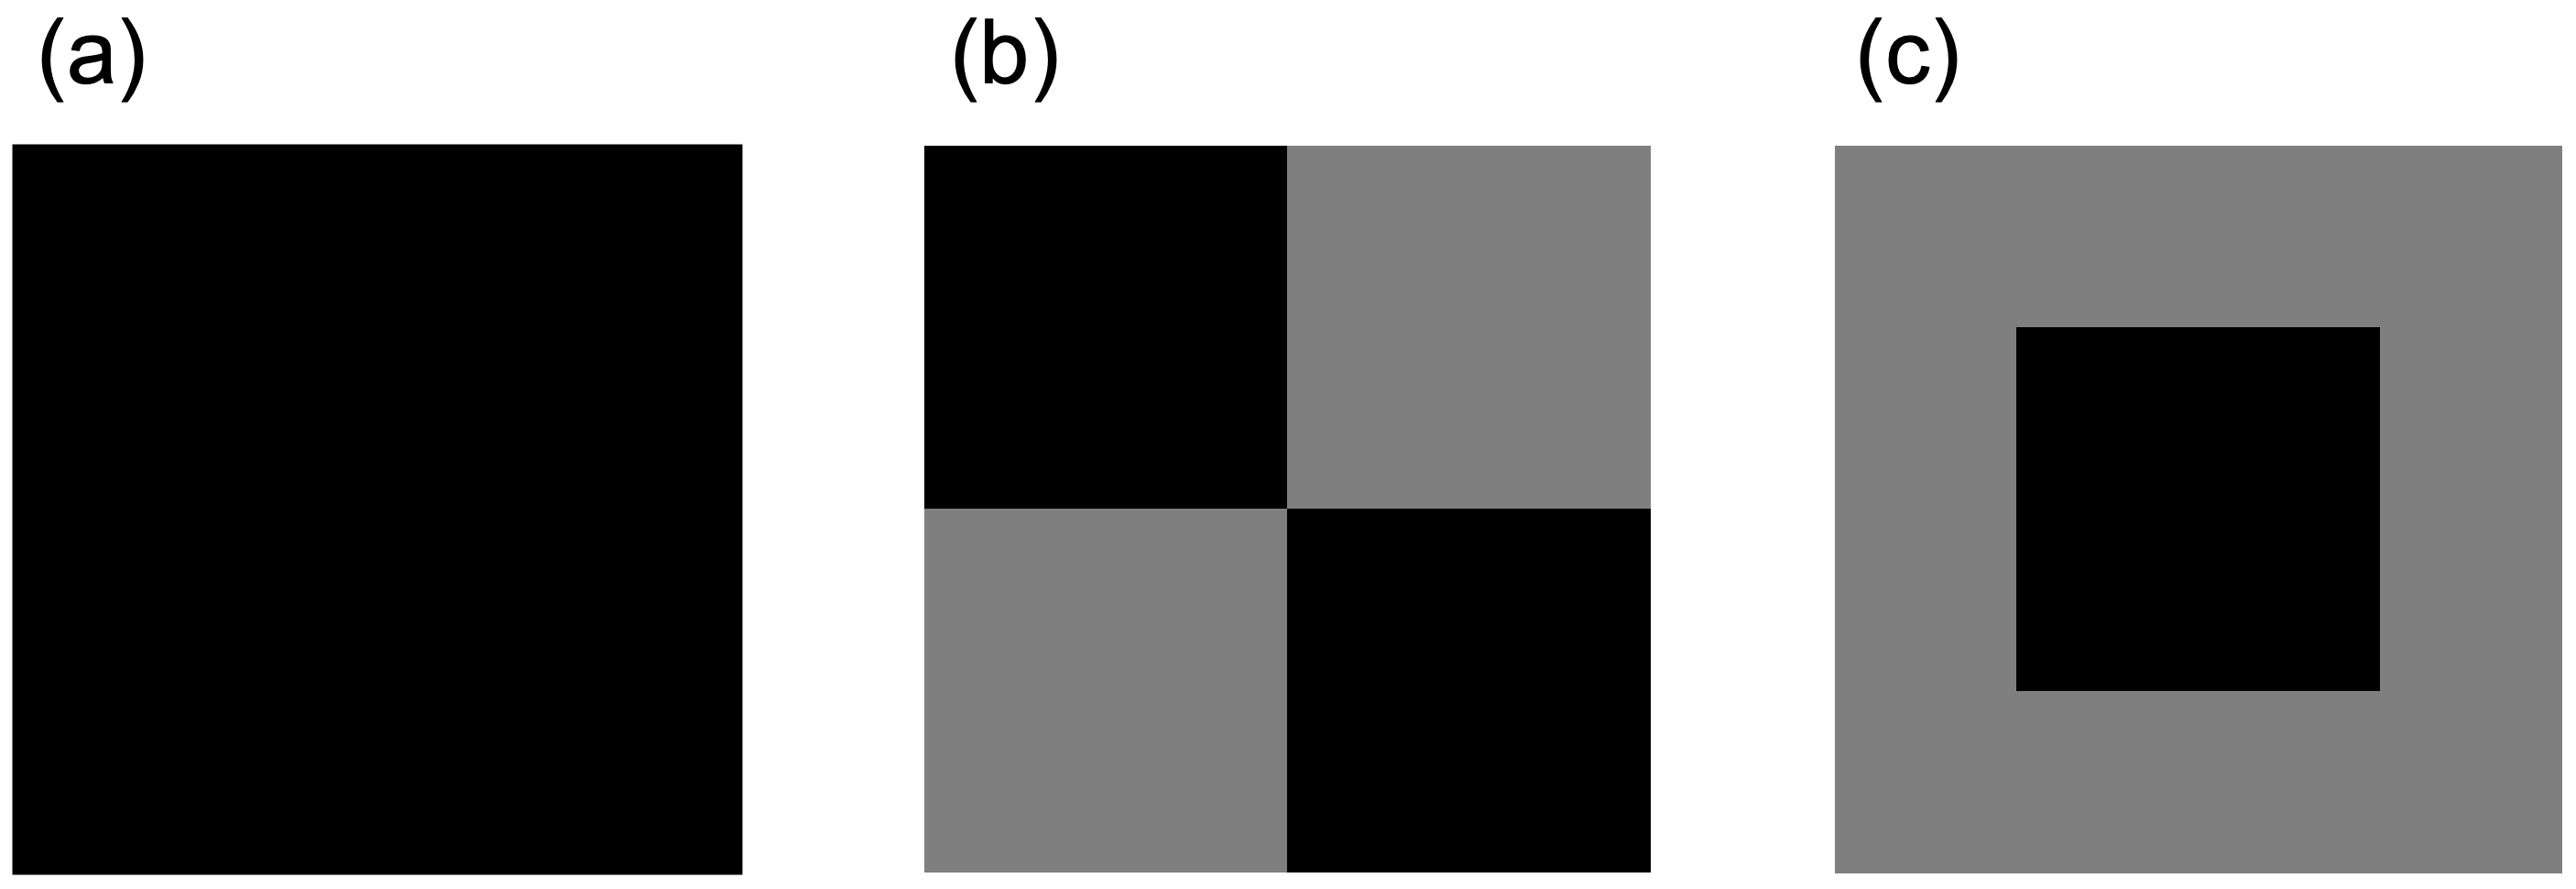
\includegraphics[width = 0.8\textwidth]{ct_images.png}
    \caption{Three objects that are to be scanned using the CT scanner described in the figure above. The black regions in this image represent the pixels with attenuation coefficient $\mu = 1$, and the gray regions represent the pixels with attenuation coefficient $\mu = 0.5$.}
    \label{fig:ctimages}
\end{figure}
\end{enumerate}

\end{document}